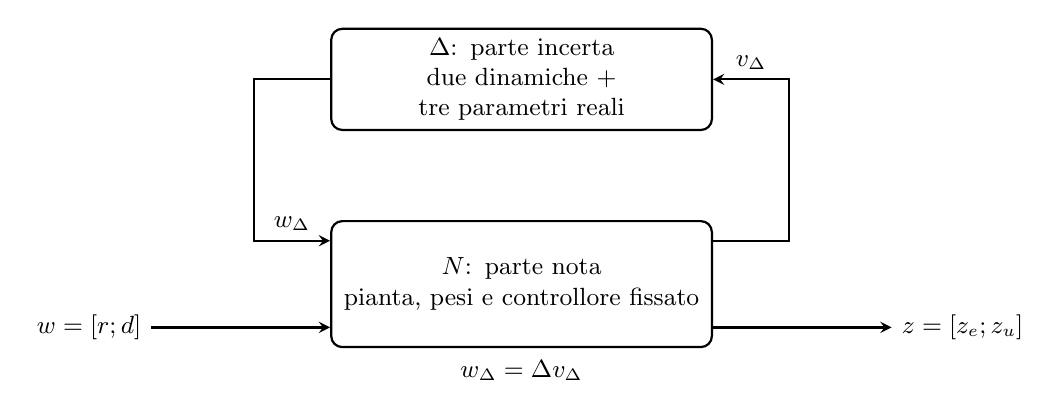
\begin{tikzpicture}[>=stealth,thick,
 b/.style={draw,rounded corners,align=center,text width=4.6cm},
 every node/.style={font=\small}]
\node[b,minimum height=1.6cm] (n) at (0,0)
 {$N$: parte nota\\pianta, pesi e controllore fissato};
\node[b,minimum height=1.2cm] (d) at (0,2.6)
 {$\Delta$: parte incerta\\due dinamiche + tre parametri reali};
\draw[->] (n.east |- 0,.55) -- (3.4,.55) -- (3.4,2.6)
 -- node[above] {$v_\Delta$} (d.east);
\draw[->] (d.west) -- (-3.4,2.6) -- (-3.4,.55)
 -- node[above] {$w_\Delta$} (n.west |- 0,.55);
\draw[->] (-4.7,-.55) node[left] {$w=[r;d]$} -- (n.west |- 0,-.55);
\draw[->] (n.east |- 0,-.55) -- (4.7,-.55) node[right] {$z=[z_e;z_u]$};
\node at (0,-1.1) {$w_\Delta=\Delta v_\Delta$};
\end{tikzpicture}
